
\chapter[Boundary value problems]{Boundary value problems for Ordinary Differential Equations}

\section{Introduction}

A boundary value problem consists in finding a solution of a
differential equation in an interval $[a,b]$ that satisfies
constraints at both ends (boundary conditions).  A typical example of
a boundary value problem is
%
\begin{equation}
  y'' = f(x,y,y'), \quad y(a) = A, \quad y(b) = B, \quad a \le x \le b.
  \label{eq:1}
\end{equation}
%
The question of the existence of solutions of problems
like~(\ref{eq:1}) is non trivial.  However, here we assume that we are
always trying to find a solution to a well posed problem, that is a
problem that has one and only one solution.

Boundary value problems describe many important physical and
engineering problems, from the sagging of a beam to the shape of the
electron orbitals in atoms.

\section{Shooting method}

We describe this method to solve boundary value problems using
equation~(\ref{eq:1}) as an example.  One natural way to attack this
problem is to solve the related initial-value problem, with a guess of
the appropriate initial value $y'(a)$. Then we can integrate the
equation to obtain the approximate solution, hoping that $y(b)=B$. If
not, then the guessed value of $y'(a)$ can be altered and we can try
again. The process is called {\bf shooting}, and there are ways of
doing it systematically.

\medskip

\noindent
Denote the guessed value of $y'(a)$ by $z$, so that the corresponding
initial value problem is
%
\begin{equation}
  y''=f(x,y,y'), \quad y(a)=A, \quad y'(a)=z, \quad a \le x \le b.\label{ivp}
\end{equation}
%
The solution of this problem is $y=y(x,z)$. The objective is to select
$z$ so that $y(b,z)=B$. We call
%
\begin{equation}
  \phi(z) \equiv y(b,z)-B ,
  \label{eq:phiz}
\end{equation}
%
so that our objective is simply to solve for $z$ the equation
%
\begin{equation}
 \phi(z)=0 \,.
 \label{eq:2}
\end{equation}
%

In general equation~(\ref{eq:2}) is nonlinear.  We can use any
numerical root finding method to solve it.  One of the most effective
is the secant method:
%
\begin{equation*}
  z_{n+1} = z_{n} - \phi(z_n) \frac{z_n - z_{n-1}}
  {\phi(z_n)-\phi(z_{n-1})} ,
  \qquad n > 1.
\end{equation*}
%
The advantage of this method is that we need only to know $\phi(z)$ in
order to apply it and that it is fairly accurate.  The disadvantage is
that we need two initial guesses $z_0$ and $z_1$ in order to start the
method.

\medskip

In the case of Newton's method, the iteration formula for $z$ is
%
\begin{equation}
 z_{n+1} = z_n-\frac{\phi(z_n)}{\phi'(z_n)}.
 \label{eq:3}
\end{equation}
%
To determine $\phi'(z)$, we can proceed in two ways.  Firstly, we
could evaluate the derivative numerically by writing
%
\begin{equation*}
  \phi'(z_n) \simeq \frac{\phi(z_n+h)-\phi(z_n)}{h}, \qquad h \ll 1.
\end{equation*}
%
A second option is to introduce
%
\begin{equation*}
  u(x,z)=\pdv{y}{z}
\end{equation*}
%
and we differentiate with respect to $z$ all the equations in
(\ref{ivp}). This becomes
%
\begin{equation*}
  u'' = f_y(x,y,y') u + f_{y'}(x,y,y') u', \quad u(a)=0, \quad u'(a)=1.
\end{equation*}
%
The last differential equation is called the \textit{first variational
  equation}.  It can integrated numerically using for $y$ and $y'$ the
values obtained by the numerical integration of equation~(\ref{ivp}).
Finally, by differentiating~(\ref{eq:2}) we obtain
%
\begin{equation*}
  \phi'(z)=u(b,z)
\end{equation*}
%
that enables us to use the Newton's method to find a root of $\phi$.

\bigskip

To summarise, the steps of the algorithm are as follows:
%
\begin{enumerate}
  %
\item Guess a value for the missing initial condition, $z_0$, and set
  the iteration counter $n$ to zero, $n=0$.
  %
\item Compute $y=y(x,z_n)$ by integrating the initial value problem
  %
  \begin{equation*}
    y''=f(x,y,y'), \quad y(a)=A, \quad y'(a)=z_n, \quad a\le x\le b.
  \end{equation*}
%
\item Compute $\phi(z_n) = y(b,z_n) - B$.  Use a nonlinear solver
  (e.g.\ Newton's or the secant method) to find a new value $z_{n+1}$
  for the missing initial condition.
%
\item If $z_{n+1}$ is not sufficiently accurate increase the iteration
  counter by one, $n \to n + 1$ and repeat steps (2-4) until
  $\phi(z_{n+1})$ is sufficiently small.
%
\end{enumerate}

\section{Finite-difference method}

Another approach to solving boundary value problems is to discretise
the derivatives that appear in the differential equation and transform
the problem in a linear system.  As an example, consider the equation
%
\begin{equation}
  y'' + p(x) y' + q(x) y = f(x), \quad y(a)=A, \quad y(b)=B,
  \quad a \le x \le b.\label{lbvp}
\end{equation}
%
We can represent the derivatives using their finite difference
approximations:
%
\begin{subequations}
  \label{er}
  \begin{align}
    y'(x_i) &= \frac{y_{i+1}-y_{i-1}}{2h} -
    \frac{h^2}{6} y'''(\xi_1), \\
    y''(x_i) &=  \frac{y_{i+1}+y_{i-1}-2 y_i}{h^2} -
    \frac{h^2}{12}y^{(4)}(\xi_2),
  \end{align}
\end{subequations}
%
where $x_i=a+i h$, $i=0,1,2,...,n+1$, $h=(b-a)/(n+1)$. Thus, the
discrete version of~(\ref{lbvp}) is the system of $n+2$ linear
algebraic equations
%
\begin{align*}
  y_0 &=A, \\
  y_{i-1} \left ( 1 - \frac{h}{2} p_i \right ) -
  y_i \left ( 2 - h^2 q_i \right ) +
  y_{i+1} \left (1 + \frac{h}{2} p_i \right )  &= h^2 f_i , \\
  y_{n+1} &=B,
\end{align*}
%
where $p_i=p(x_i)$, $q_i=q(x_i)$, $f_i=f(x_i)$.  This can be solved as
such or reduced to an $n \times n$ system.  For example, if $n=4$, the
corresponding matrix form is given by
%
\begin{equation*}
  \begin{pmatrix}
    -2 + h^2 q_1 & 1 + \frac{h}{2} p_1 & 0 & 0 \\
    1 - \frac{h}{2} p_2 & -2  + h^2 q_2 & 1 + \frac{h}{2} p_2 & 0\\
    0 & 1 - \frac{h}{2} p_3 & -2  + h^2 q_3 & 1 + \frac{h}{2} p_3 \\
    0 & 0 & 1 - \frac{h}{2} p_4 & -2  + h^2 q_4
  \end{pmatrix}
  \begin{pmatrix} y_1\\ y_2\\ y_3\\ y_4 \end{pmatrix} =
  \begin{pmatrix} F_1\\ F_2\\ F_3\\ F_4 \end{pmatrix}
\end{equation*}
%
with
%
\begin{align*}
  & &  F_1 & = h^2 f_1 - A (1 - \frac{h}{2} p_1), &
  F_2 & = h^2 f_2, \\
  & &  F_3 & = h^2 f_3, & F_4 & = h^2 f_4 - B(1 + \frac{h}{2} p_4).
\end{align*}
%
This system is tridiagonal and can be solved by a special form of the
Gaussian elimination algorithm. In the general case, we have an
$n\times n$ system
%
\begin{equation}
  T \boldsymbol{y} = \boldsymbol{F},
  \label{eq:5}
\end{equation}
%
where $T$ is a tridiagonal $n\times n$ matrix,
$\boldsymbol{y}=(y_1,...,y_n)^T$ and $\boldsymbol{F}=(F_1,...,F_n)^T$.

To analyse the error induced by the representation~(\ref{er}) of the
derivatives we introduce an error vector $(e_1,...,e_n)$, where
$e_i=y(x_i)-y_i$, $i=1,\ldots,n$ and $y(x)$ is assumed to be the exact
solution.  Substituting into the finite difference
representation~(\ref{eq:5}) of equation~(\ref{lbvp}), we obtain the
system
%
\begin{equation*}
  T \be = h^4 \boldsymbol{G}
\end{equation*}
%
where $\boldsymbol{G}$ is a constant vector.   If $\det T \ne 0$, we have
%
\begin{equation*}
  \boldsymbol{e}=h^4T^{-1}\boldsymbol{G}.
\end{equation*}
%
We can use this relation to show that the error is $O(h^2)$ [sic] as
$h \to 0$.

\section{The Ritz method}

The Ritz, Galerkin, Square Least methods are used widely on problems
in which it is required to determine an unknown function. Of course,
boundary value problems for differential equations are in this
category. Suppose we are confronted with a problem of the form
%
\begin{equation}
  \mathcal{L} u(x)=f(x)
\end{equation}
%
in which $\mathcal{L}$ is the linear operator
%
\begin{equation}
  \mathcal{L} u=-\dv{}{x} \left[ p(x) \dv{u}{x} \right ] + q(x)u = f(x).
\end{equation}
%
Here $f(x)$ is a given function and $u(x)$ is is the function to be
determined from the equation and boundary conditions
%
\begin{equation}
  u(a)=0, \qquad u(b)=0.
\end{equation}
%
We assume that $p(x)\ge p_0>0$, $q(x)\ge 0$ for $x\in [a,b]$. This
means that the operator $\mathcal{L}$ is symmetric and positive
definite in the real Hilbert space $L_2[a,b]$ since, using the
integration by parts, we have
%
\begin{align*}
  <\mathcal{L}u,u> & = \mint{a}{b}{\mathcal{L} u \cdot u}{x} \\
  & = -\mint{a}{b}{(p u')'u}{x} + \mint{a}{b}{q u^2}{x} \\
  & = \mint{a}{b}{p(u')^2}{x} + \mint{a}{b}{q u^2}{x} \ge 0
\end{align*}
%
for arbitrary $u$. The quantity $<\mathcal{L}u,u>$ is called the
energy of the element $u$ relative the operator $\mathcal{L}$.

\noindent Consider a linear quadratic functional
%
\begin{subequations}
  \label{fun}
  \begin{align}
    J(u) & = <\mathcal{L}u,u>-2<f,u> \\
         & = \mint{a}{b}{p(u')^2}{x} + \mint{a}{b}{q u^2}{x} -2 \mint{a}{b}{f
         u}{x}.
  \end{align}
\end{subequations}
%
A theorem states that if the equation $\mathcal{L}u(x)=f(x)$ has a
solution $u_0$, this solution minimises the functional
$J(u)$. Conversely, if there exists an element $u_0$ that minimises
the functional $J(u)$, this element satisfies the equation
$\mathcal{L}u(x)=f(x)$.  The proof is based on the ability to reduce
the functional $J(u)$ to the form
%
\begin{equation*}
  J(u)=<\mathcal{L}(u-u_0),u-u_0>-<\mathcal{L}u_0,u_0>,
\end{equation*}
%
and then analysing the function
%
\begin{align*}
 g(t) & = J[u_0(x)+t v(x)] \\
      & = <\mathcal{L}u_0,u_0> + 2t<\mathcal{L}u_0,v> +
      t^2<\mathcal{L} v,v> - 2<f,u_0> - 2t<f,v>.
\end{align*}
%
The basic idea of the Ritz method consists in replacing the boundary
value problem for $\mathcal{L}u(x)=f(x)$ by the problem of minimising
the functional $J(u)$. Suppose we select basis functions $u_1$,
$u_2$,...,$u_n$,... in $L_2[a,b]$.  Hence, we seek a solution of the
form
%
\begin{equation}
  u_n(x)=\sum_{m=1}^n c_m u_m(x),\label{rsol}
\end{equation}
%
where $c_1$, $c_2$,...,$c_n$ are unknown constants.  Substituting this
sum into the functional $J(u)=<\mathcal{L}u,u>-2<f,u>$, we obtain
%
\begin{equation}
  J(u_n)=J(c_1,c_2,...,c_n)=\sum_{m,k=1}^n c_m c_k<\mathcal{L}u_m,u_k>-
  2\sum_{m=1}^n c_m<f,u_m>,
\end{equation}
%
which is a quadratic form with respect to the unknown constants
$c_1,c_2,...,c_n$.  Looking for a minimum element of
$J(u_n)=J(c_1,c_2,...,c_n)$, we require that
%
\begin{equation}
  \pdv{}{c_m} J(c_1,c_2,...,c_n)=0, \qquad m=1,2,...,n.
\end{equation}
%
Thus, we come to the linear $n\times n$ system of algebraic equations
for the unknown constants $c_1$, $c_2$,...,$c_n$
%
\begin{equation}
  \sum_{m=1}^nc_m<\mathcal{L}u_m,u_k>=<f,u_k>,~~~~~k=1,2,...,n,\label{sys}
\end{equation}
%
which is called the Ritz system.  After we have found the unknown
constants $c_1$, $c_2$,...,$c_n$, the expression (\ref{rsol}) gives us
an approximate solution.

\section{The collocation method}

\subsection{Introduction}

The method of collocation can be used to tackle many problems in the
numerical analysis of ordinary and partial differential equations.
Here we give a general description of this method that can be adapted
easily to the solution of a boundary value problem for an ordinary
differential equation.

Suppose that we have a linear operator $\mathcal{L}$ (for example, a
linear differential equation) that acts on a space of functions.  We
wish to solve the equation
%
\begin{equation}
  \mathcal{L} u(x) = w(x) ,
  \label{cwk4.eq:1}
\end{equation}
%
where $w(x)$ is a known function and $u(x)$ is the solution we are
looking for.  We indicate with
%
\begin{equation*}
  \{v_1(x), v_2(x), \ldots, v_n(x)\}
\end{equation*}
%
a set of $n$ known functions (\textit{basis functions}) and we write
the (unknown) solution of equation~(\ref{cwk4.eq:1}) as
%
\begin{equation}
  u(x) = \sum_{j=1}^n c_j v_j(x) ,
  \label{cwk4.eq:2}
\end{equation}
%
where the coefficients $c_j$ are (at this stage) unknown.  In general
$u(x)$ written as in equation~(\ref{cwk4.eq:2}) cannot be an exact
solution of equation~(\ref{cwk4.eq:1}).  However, we can find a set of
coefficients $\{c_j\}$ such that~(\ref{cwk4.eq:2}) is a good
approximation of the solution of the equation~(\ref{cwk4.eq:1}).

\medskip

\noindent \textbf{Remark} - Note that the series solution of a
differential equation falls into this class of methods.   In that case
the functions $v_j(x)=x^j$, with $j=0,1,2,\ldots,n$ and the
coefficients $c_j$ of the expansion are determined by requiring that
equation~(\ref{cwk4.eq:1}) is satisfied at each order in $x$.

\subsection{The norm method}

There are various ways of defining ``good approximation''.  As a first
example, consider the boundary value problem
%
\begin{equation}
  u''(x) - u(x) = 0 \, , \qquad
  u(0) = 1, \quad u(1) = e.
  \label{cwk4.eq:4}
\end{equation}
%
We wish to find an approximate solution to this problem using as basis
the functions
%
\begin{equation*}
  v_0(x) = 1 , \quad v_1(x) = x \quad \text{and} \quad v_2(x) = x^2,
\end{equation*}
%
and write the approximate solution of equation~(\ref{cwk4.eq:4}) as a
polynomial of order two:
%
\begin{equation}
  u^{(a)}(x) = c_0 v_0(x) + c_1 v_1(x) + c_2 v_2(x) =
  c_0 + c_1 x + c_2 x^2 .
 \label{cwk4.eq:5}
\end{equation}
%
It is clear that there are no values of the constants $c_j$ that can
make $u^{(a)}(x)$ as defined in equation~(\ref{cwk4.eq:5}) equal to
the exact solution of equation~(\ref{cwk4.eq:4}),
%
\begin{equation}
  u^{(e)}(x) = e^x
  \label{cwk4.eq:3}
\end{equation}
%
for all values of $x$.  However, we can attempt to find some values of
these parameters that minimise the error in approximating $u^{(e)}(x)$
with $u^{(a)}(x)$.  There are many different measures of the error of
the approximation.  For example, we could require that the
coefficients $c_j$ are such that

\begin{enumerate}
  %
\item $u^{(a)}(x)$ satisfies the boundary conditions, i.e.\ $u^{(a)}(0)=1$ and $u^{(a)}(1) = e$.
  %
\item $u^{(a)}(x)$ satisfies as well as possible
  equation~(\ref{cwk4.eq:4}) in the sense that
  %
  \begin{equation}
    F(c_j) \equiv
    \left \| \dv[2]{}{x} u^{(a)}(x) - u^{(a)}(x) \right \|_2^2 =
    \mint{0}{1}{\left [ \dv[2]{}{x} u^{(a)}(x) - u^{(a)}(x)
    \right ]^2}{x}
    \label{eq:10}
  \end{equation}
  %
  is as small as possible.  A criterion (distantly?) related to this
  is used in the finite element method to solve partial differential
  equations.
  %
\end{enumerate}

\begin{figure}
  \centerline{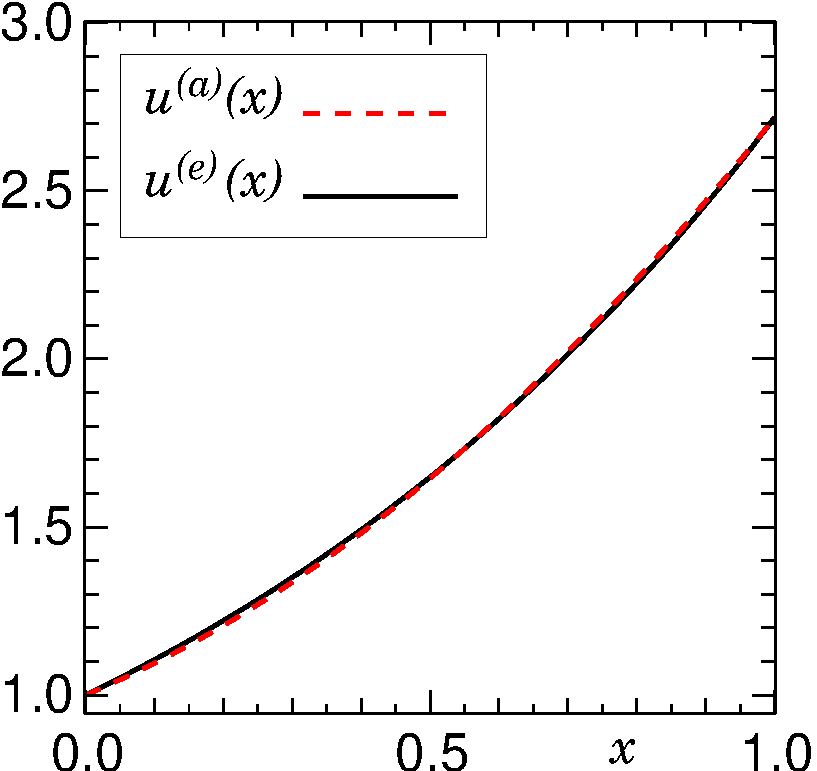
\includegraphics[width=80mm]{figures/ColloEner}}
  \caption{\label{fig:ColloEner} \it Graphs of the exact
    [Eq.~(\ref{cwk4.eq:3})] and approximate [Eq.~(\ref{eq:12})]
    solution of the boundary value problem~(\ref{cwk4.eq:4}).}
\end{figure}

The left boundary condition fixes $c_0$:
%
\begin{equation}
  u^{(a)}(0) = c_0 = 1 .
  \label{eq:9}
\end{equation}
%
The right boundary condition gives a relation between $c_1$ and $c_2$:
%
\begin{equation}
  u^{(a)}(1) = c_0 + c_1 + c_2 = e \implies c_1 = e - 1 - c_2 .
  \label{eq:8}
\end{equation}
%
Substituting~(\ref{eq:9}) and~(\ref{eq:8}) into~(\ref{cwk4.eq:4})
gives that $F(c_j)$ defined by~(\ref{eq:10}) is
%
\begin{equation}
  F(c_2) = \frac{47}{10} c_2^2 - \frac{13}{6}(1+e)c_2 + \frac{1+e+e^2}{3} .
  \label{eq:11}
\end{equation}
%
We solve for $c_2$ by requiring that $F(c_2)$ is as small as possible,
i.e.\ that the derivative of $F(c_2)$ with respect to $c_2$ is zero.
Differentiating~(\ref{eq:11}) we obtain
%
\begin{equation*}
 \dv{F}{c_2} = \frac{47}{5} c_2 - \frac{13}{6}(1+e) = 0 \implies
 c_2 = \frac{65}{282}(1+e) ,
\end{equation*}
%
so that from equation~(\ref{eq:8}) we have
%
\begin{equation*}
  c_1 = \frac{217 e - 347}{282}
\end{equation*}
%
and the approximate solution of the boundary value
problem~(\ref{cwk4.eq:4}) is
%
\begin{equation}
  u^{(a)}(x) = 1 + \frac{217 e - 347}{282} x + \frac{65}{282}(1+e) x^2 .
  \label{eq:12}
\end{equation}
%
The graphs of the approximate and exact solutions are shown in
Figure~\ref{fig:ColloEner}: the match is pretty impressive for a three
node approximation.

\subsection{The collocation method}

In the \textit{collocation} method we substitute the approximate
solution~(\ref{cwk4.eq:2}) in~(\ref{cwk4.eq:1}),
%
\begin{equation*}
  \mathcal{L} \sum_{j=1}^n c_j v_j(x) = w(x) \implies
  \sum_{j=1}^n c_j \mathcal{L} v_j(x) = w(x) ,
\end{equation*}
%
and we require that this equation should be satisfied at a set of $n$
\textit{collocation points} $\{x_j\}$, i.e.\ that the coefficients
$c_j$ are the solution of the system of linear equations
%
\begin{equation*}
  \sum_{j=1}^n c_j \mathcal{L} v_j(x_k) = w(x_k) , \qquad k=1,2,\ldots,n.
\end{equation*}
%
Note that the values of the basis functions $v_j(x)$ at the
collocation points $x_k$ should be such that the matrix of the
coefficients of this system is non-singular.

\begin{figure}
  \centerline{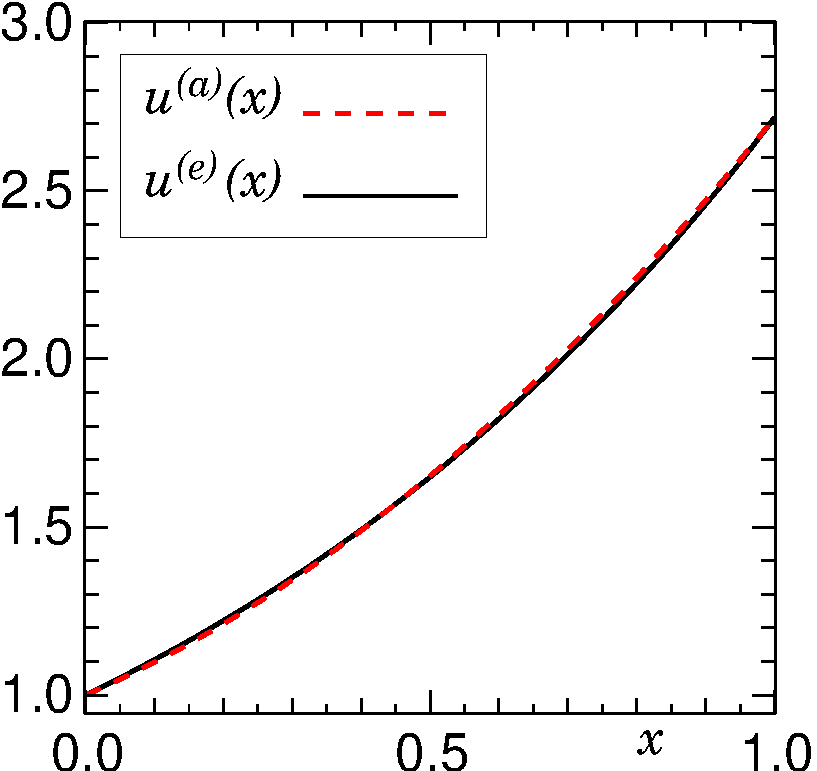
\includegraphics[width=80mm]{figures/Collocation}}
  \caption{\label{fig:Collocation} \it Graphs of the exact
    [Eq.~(\ref{cwk4.eq:3})] and approximate [Eq.~(\ref{eq:13})]
    solution of the boundary value problem~(\ref{cwk4.eq:4}).}
\end{figure}

Once again consider as an example the boundary value
problem~(\ref{cwk4.eq:4}) and write the approximate solution as in
equation~(\ref{cwk4.eq:5}).  We require that it should satisfy the
boundary conditions as in equations~(\ref{eq:9}) and~(\ref{eq:8}), so
that the approximate solution is now given by
%
\begin{equation*}
  u^{(a)}(x) = 1 + (e-1-c_2) x + c_2 x^2 .
\end{equation*}
%
Finally, we require that this function should satisfy the differential
equation~(\ref{cwk4.eq:4}) at $x=1/2$.  Taking into account that
%
\begin{equation*}
 \dv[2]{}{x} u^{(a)}(x) = 2 c_2
\end{equation*}
%
we have that this requirement is equivalent to
%
\begin{equation*}
  2 c_2 - \left [ 1 + (e-1-c_2) \frac{1}{2} +
    c_2 \left ( \frac{1}{2} \right )^2 \right ] = 0 \implies
  c_2 = \frac{2}{9}(1+e) \implies c_1 = \frac{7 e - 11}{9}
\end{equation*}
%
so that the approximate solution is given by
%
\begin{equation}
  u^{(a)}(x) = 1 + \frac{7 e - 11}{9} x + \frac{2}{9}(1+e) x^2 .
  \label{eq:13}
\end{equation}
%
The graphs of the approximate and exact solutions are shown in
Figure~\ref{fig:Collocation}: the match is pretty impressive for a
three node approximation and is comparable, but different, from that
in Figure~\ref{fig:ColloEner}.

\smallskip

\noindent \textbf{Remark} - In general it is not advisable to use as
basis functions the powers of $x$ or a uniformly spaced set of nodes.
Orthogonal polynomials (like the Legendre and the Chebyschev
polynomials) and non-uniform grids (e.g.\ Gauss-Lobatto grids) give
more accurate and numerically stable results.


\section*{Further reading}

Topics covered here are also covered in
\begin{itemize}
\item Chapter 11 of Linz \& Wang, \textit{Exploring Numerical Methods}
  (QA297 LIN),
\item Chapter 8 of Kincaid \& Cheney, \textit{Numerical Analysis}
  (QA297 KIN),
\item Chapter 13 (and to some extent 14) of S{\"u}li \& Mayers,
  \textit{An Introduction to Numerical Analysis} (not in library).
\end{itemize}
